%%%%%%%%%%%%%%%%%%%%%%%%%%%%%%%%%%%%%%%%%%%%%%%%%%%%%%%%%%%%%%%%%%%%%%%%%%%%%%%%
\chapter[Explosão Digital]{Explosão Digital\\\large\textit{Por que está
acontecendo e o que está em jogo?}}
\label{cap1:exp-dig}

Este livro não é sobre computadores. É sobre a sua vida e a minha. É sobre como
o terreno embaixo de nós mudou de maneiras fundamentais. Todos nós sabemos que
isso está acontecendo. Vemos isso ao nosso redor todos os dias. Todos nós
precisamos entender isso melhor.

A explosão digital está mudando tudo. Neste livro, falamos sobre o que está
acontecendo e como. Explicamos a tecnologia em si --- porque ela cria tantas 
surpresas e porque as coisas muitas vezes não funcionam como esperamos. Também 
é sobre as coisas que a explosão da informação está destruindo: pressupostos
antigamente dados como consolidados sobre nossa privacidade, sobre nossa
identidade e sobre quem controla nossas vidas. É sobre como chegamos a esse
ponto, o que estamos perdendo e o que ainda resta para a sociedade ter a chance
de corrigir.

A explosão digital está criando oportunidades e riscos. Muitos deles 
desaparecerão em uma década, resolvidos de uma forma ou de outra. Governos, 
corporações e outras autoridades estão aproveitando o caos, e a maioria de nós 
nem mesmo percebe que isso está acontecendo. No entanto, todos nós temos
interesse no resultado. Além da ciência, da história, da lei e da política, este
livro é um alerta. As forças que moldam o seu futuro são digitais, e você 
precisa entendê-las.

Este livro trata das histórias que ouvimos e lemos todos os dias. Histórias que 
se referem ao impacto profundo e muitas vezes inesperado que a tecnologia 
digital está tendo em nossas vidas. Vamos começar com a história de Nicolette 
Vartuli.

Nicolette não conseguia entender porque não conseguiu o emprego. Ela é uma
estudante universitária com GPA de 3,5\footnote{[NT] GPA, do inglês
\ingles{Grade Point Average}, é um número que indica o rendimento, o
aproveitamento acadêmico nas universidades americanas. É equivalente ao CR
(coeficiente de rendimento) utilizado nas universidades brasileiras. O GPA é
calculado, grosso modo, como uma média ponderada das notas de cada uma das
disciplinas e, em geral, varia de 0 a 4. Para saber mais:
\url{https://en.wikipedia.org/wiki/Grading_in_education}.}, 
se preparou para a entrevista no banco de investimentos e se manteve
positiva durante todo o processo. Ela manteve a cabeça erguida, sorriu e falou
com confiança. Mas quando a empresa entrou em contato com a resposta, foi uma má
notícia. Ela não seguiria adiante no processo de contratação\footnote{Drew
Harwell, ``A Face-Scanning Algorithm Increasingly Decides Whether You Deserve
the Job,'' \textit{Washington Post}, November 6, 2019, \url{https://www.washingtonpost.com/technology/2019/10/22/ai-hiring-face-scanning-algorithm-increasingly-decides-whether-you-deserve-job/}.}. 

Nicolette queria saber o que ela havia feito de errado, mas ninguém pôde
explicar o motivo dela ter sido rejeitada --- porque ninguém realmente sabe.
Ela foi entrevistada por um computador que usava um software de inteligência
artificial da HireVue para avaliar sua adequação. Esse software a rejeitou não
porque ela não tinha alguma qualificação específica, mas porque, como a HireVue
afirmava, o software conseguia detectar padrões em pessoas que tinham sucesso no
trabalho --- e o que observou em Nicolette não correspondia. É fácil entender
ser rejeitado porque você não tem três anos de experiência exigida ou alguma
habilidade específica. Isso é diferente. E assustador --- especialmente porque
não há nenhuma explicação sobre o que o software estava procurando. E pode ser
que nenhuma explicação pudesse ser oferecida, mesmo que a HireVue estivesse
disposta a divulgar seus algoritmos proprietários (ela não está.)

As empresas gostam dessa nova tecnologia. É mais barata e eficiente do que 
entrevistas humanas. Na verdade, a HireVue, apenas uma das muitas fornecedoras, 
já realizou mais de 10 milhões de entrevistas. Muitos candidatos, por outro 
lado, não gostam desses assistentes de contratação automatizados. Não é apenas o 
fato de se sentir desumanizado ao ser julgado por uma máquina. As empresas que 
oferecem esse serviço argumentam que, ao usar a tecnologia, mais pessoas podem 
conseguir entrevistas, e a probabilidade de preconceito inerente por parte dos
entrevistadores é reduzida. Eles afirmam que a tecnologia está abrindo
oportunidades, não limitando-as --- mas como podemos ter certeza disso?

A antipatia instintiva à triagem automatizada de empregos não é causada porque
as pessoas não querem que os computadores tomem decisões críticas em situações
de risco à vida. Muitas dessas decisões são tomadas por computadores hoje em
dia, por exemplo: os sistemas de avião e de radioterapia são em grande parte 
automatizados; computadores agora superam radiologistas altamente treinados na 
detecção de tumores de câncer em mamografias\footnote{Scott Mayer McKinney et
al., ``International Evaluation of an AI System for Breast Cancer Screening,''
\textit{Nature} 577, no. 7788 (January 2020): 89--94,
\url{https://doi.org/10.1038/s41586-019-1799-6}.}. Alguém iria preferir
avaliadores humanos menos precisos? Mas os julgamentos da HireVue são de um tipo
diferente. O programa tomou uma decisão sobre a humanidade de Nicolette. Decidiu
que ela não era o tipo de pessoa que a empresa deveria contratar, e fez isso sem
explicar a ela ou a qualquer outra pessoa qual seria o tipo de pessoa adequada
para a contratação e como Nicolette não se encaixava.

Muitos outros sistemas estão fazendo julgamentos semelhantes em outros domínios
humanos hoje em dia. Juízes consultam computadores para avaliar o risco de réus 
criminais não comparecerem aos seus julgamentos --- novamente comparando os 
indivíduos com outros que foram presos no passado e tiveram o benefício de 
evitar a detenção antes do julgamento\footnote{Julia Angwin et al., ``Machine
Bias,'' \textit{ProPublica}, May 23, 2016,
\url{https://www.propublica.org/article/machine-bias-risk-assessments-in-criminal-sentencing}.}. Agentes
imobiliários usam computadores para avaliar quais potenciais inquilinos
provavelmente serão devedores\footnote{Elizabeth Fernandez, ``Will Machine
Learning Algorithms Erase the Progress of the Fair Housing Act?''
\textit{Forbes}, November 17, 2019,
\url{https://www.forbes.com/sites/fernandezelizabeth/2019/11/17/will-machine-learning-algorithms-erase-the-progress-of-the-fair-housing-act/}.}.

A maioria desses sistemas é proprietária, e as empresas que os desenvolvem não 
precisam divulgar como eles funcionam. E afinal, argumentam eles,
entrevistadores humanos também não podem ser considerados como um padrão de
julgamento imparcial. Eles estão sujeitos a todo tipo de preconceitos e
tendências infelizes. É por isso que as audições para músicos instrumentais
agora são comumente realizadas sem que os ouvintes vejam os candidatos: quando
os intérpretes podiam ser vistos, as mulheres eram sistematicamente julgadas de
forma mais rigorosa do que os homens\footnote{Claudia Goldin and Cecilia Rouse,
``Orchestrating Impartiality: The Impact of `Blind' Auditions on Female
Musicians,'' \textit{The American Economic Review} 90, no. 4 (September 2000),
\url{https://pubs.aeaweb.org/doi/pdfplus/10.1257/aer.90.4.715}.}. Ao comparar as
habilidades dos candidatos nas entrevistas às dos trabalhadores existentes, a
HireVue afirma estar eliminando a parte mais falível do sistema. São os
recrutadores humanos, diz a HireVue, que são a ``caixa-preta final''. Talvez ---
exceto que a HireVue afirma estar combinando os candidatos ao perfil dos
melhores funcionários atuais do banco. Como alguém saberia se o software está
simplesmente replicando, agora automaticamente, todos os preconceitos que deram
ao banco a força de trabalho que ele tem agora?

O que torna toda essa história particularmente importante não é apenas o fato de
Nicolette ter sido considerada inadequada por uma máquina mas, sim, o fato de
que ninguém --- nem um gerente de recursos humanos, nem mesmo um programador ---
informou ao software da HireVue quais critérios usar. Ele determinou tudo
sozinho. O software assistiu a vídeos de funcionários existentes e escolheu seus
próprios critérios.

A história da candidatura de emprego rejeitada de Nicolette é o que chamamos de 
uma ``história de bits''. Não é apenas uma história de busca de emprego; é uma
história sobre a coleta, armazenamento, análise, transmissão e uso de trilhões
de trilhões de trilhões de $0$s e $1$s individuais. Ao analisar cuidadosamente
essas histórias, podemos entender não apenas a tecnologia por trás delas, mas
também suas implicações e riscos.

\begin{tcolorbox}
A ``transparência algorítmica'' é o princípio de que devemos saber como os
computadores estão tomando decisões sobre nós. Nas palavras da EPIC
(\ingles{Electronic Privacy Information Center} --- Centro de Informações sobre
Privacidade Eletrônica): ``O público tem o direito de conhecer os processos de
dados que impactam suas vidas, para que possam corrigir erros e contestar
decisões tomadas por algoritmos.''\footnote{``Algorithmic Transparency: End
Secret Profiling,'' \textit{Electronic Privacy Information Center}, March 1,
2020, \url{https://epic.org/algorithmic-transparency/}.}
\end{tcolorbox}

Os bits representavam a imagem de Nicolette enquanto fluíam de seu próprio
computador para o da HireVue, por meio de fios, cabos e provavelmente vários
tipos de ondas de rádio. Os bits foram desmontados, remontados e analisados
pelos programas da HireVue. Eles foram de alguma forma comparados a trilhões de
trilhões de trilhões de outros bits que representam vídeos de outras pessoas e,
em seguida, um único bit, um simples sim ou não, foi emitido: continuar para a
próxima etapa do processo de contratação ou rejeitar imediatamente. Esse bit foi
um $0$ para Nicolette, e foi tudo o que ela ouviu da empresa. Mas a HireVue
manteve todos os bits da entrevista malsucedida de Nicolette; ela teve que ceder
seus direitos sobre eles para conseguir a entrevista em primeiro lugar.

Essas novas tecnologias interagem de maneiras estranhas com os padrões em
evolução de privacidade, práticas de comunicação e legislação criminal. A
história de Nicolette, embora importante para ela, é apenas uma das milhares de
histórias de bits que poderiam ser contadas sobre qualquer um de nós. Todos os
dias encontramos consequências inesperadas do fluxo de dados que não poderiam
ter ocorrido há apenas alguns anos atrás.

Quando você terminar de ler este livro, você verá o mundo de uma maneira 
diferente. Você ouvirá uma história de um amigo ou em um noticiário e dirá a si 
mesmo: ``Isso é, na verdade, uma história de bits'', mesmo que ninguém mencione
nada digital. Os movimentos de objetos físicos e as ações de seres humanos de 
carne e osso são apenas a superfície. Para entender o que realmente está 
acontecendo, você precisa enxergar o mundo virtual, o sinistro fluxo de bits 
que está direcionando os eventos de nossas vidas.

Este livro é seu guia para este novo mundo.


%%%%%%%%%%%%%%%%%%%%%%%%%%%%%%%%%%%%%%%%
\section{A explosão de bits e tudo mais}
\label{cap1:exp-dig-bits}

O mundo mudou muito repentinamente. Quase tudo está armazenado em algum 
computador. Registros judiciais, compras de supermercado, preciosas fotos de 
família e filmes de Hollywood inestimáveis, programas de televisão sem 
sentido\ldots\ Os computadores contêm uma quantidade enorme de coisas que não 
são úteis atualmente, mas que alguém acredita que possam ser úteis algum dia. 
Tudo está sendo reduzido a 0s e 1s, ``bits''. Os bits são armazenados em discos
de computadores domésticos, nos centros de dados de grandes corporações e 
agências governamentais. Muitos dos discos nem mesmo são objetos redondos e 
giratórios --- são um tipo diferente de mídia de armazenamento, chamados 
``discos'' por razões históricas. A maioria dos discos hoje em dia está ``na
nuvem'' --- apenas um nome sofisticado para discos pertencentes a grandes 
empresas como a Amazon, alugados para quem precisa de espaço para armazenar 
coisas. Os discos podem armazenar tantos bits que não há necessidade de escolher 
o que deve ser lembrado.

\begin{tcolorbox}
``Bit'' é uma abreviação de ``dígito binário''. O sistema de numeração binária
utiliza apenas dois algarismos, 0 e 1, em vez dos dez algarismos 0, 1, 2, 3, 4,
5, 6, 7, 8 e 9 usados no sistema decimal. A primeira declaração clara dos
princípios da notação binária foi feita por Gottfried Wilhelm Leibniz em 1679.
\end{tcolorbox}

Tanta informação digital, desinformação, dados e lixo estão sendo armazenados 
que a maioria disso será visto apenas por computadores, nunca pelos olhos 
humanos. E os computadores estão ficando cada vez melhores em extrair 
significado de todos esses bits --- encontrando padrões que às vezes resolvem
crimes, diagnosticam doenças e fazem sugestões úteis --- e às vezes revelam
coisas sobre nós que não esperávamos que os outros soubessem.

A história de Edward Snowden, que vazou milhares de documentos altamente
secretos do governo em 2013, é uma história de bits. Ele levou os documentos 
para fora dos Estados Unidos em seu laptop; apenas alguns anos antes, ele
precisaria carregar centenas de quilos de papel. E tudo o que ele revelou estava
relacionado à vigilância eletrônica do governo, levantando questões fundamentais
sobre os \ingles{trade-offs} entre privacidade e segurança.

O impedimento do 737 Max em 2019 não foi apenas uma história de avião. Foi 
também uma história de bits. Os motores dos modelos anteriores do 737 haviam 
sido movidos, alterando a distribuição de peso da aeronave; o software 
desenvolvido para processar dados dos sensores e controlar automaticamente os 
movimentos do avião não funcionou como pretendido\footnote{Benjamin Zhang, ``The
Boeing 737 Max Is Likely to Be the Last Version of the Best-Selling Airliner of
All Time,'' \textit{Business Insider}, March 19, 2019, \url{https://www.businessinsider.com/boeing-737-max-design-pushed-to-limit-2019-3.}}.

Mas não são apenas os eventos de importância global que são histórias de bits; 
são as histórias do dia a dia da vida comum. A experiência perturbadora da 
corredora recreativa Rosie Spinks é uma história de bits. Spinks usava um 
aplicativo em seu telefone para rastrear suas rotas e tempos, e ela pensava que 
sua localização estava sendo mantida em segredo porque ela tinha ativado a 
configuração de ``Privacidade Aprimorada'' do aplicativo. Apenas quando
estranhos começaram a ``curtir'' seus treinos enquanto ela estava viajando para
o exterior, ela percebeu que ``Privacidade Aprimorada'' na verdade significava
``contar para homens aleatórios sobre meus treinos se eu estiver na lista dos
melhores''. O aplicativo de condicionamento físico também era um aplicativo de
rede social, e os dados de Rosie estavam sendo comercializados\footnote{Rosie
Spinks, ``Confused About How to Use Strava Safely? You Are Not Alone,''
\textit{Quartz}, January 29, 2018, \url{https://qz.com/1191431/strava-privacy-concerns-here-
is-how-to-safely-use-the-app/.}}.

Uma vez que algo está em um computador, pode se replicar e se mover pelo mundo 
em um piscar de olhos. Fazer um milhão de cópias perfeitas leva apenas um 
instante --- cópias de coisas que queremos que todos no mundo vejam e também 
cópias de coisas que não eram para ser copiadas de jeito nenhum.

A explosão digital está mudando o mundo tanto quanto a impressão já fez --- e 
algumas das mudanças estão nos pegando desprevenidos, desmontando nossas 
suposições sobre como o mundo funciona.

A explosão digital pode parecer benigna, divertida ou até mesmo utópica. Em vez 
de enviar fotos pelo correio para a vovó, compartilhamos imagens de nossos 
filhos no Instagram. Assim, não apenas a vovó pode vê-las, mas também os amigos 
da vovó e qualquer outra pessoa. Desfrutamos dos benefícios, mas quais são os 
riscos? As fotos são fofas e inofensivas. Mas suponha que um turista tire uma 
foto de férias e você apareça ao fundo, em um restaurante onde ninguém sabia que 
você estava jantando. Se o turista enviar a foto e torná-la pública, o mundo 
inteiro poderá saber onde você estava e quando esteve lá. O reconhecimento 
facial, que há apenas alguns anos estava além das capacidades dos computadores, 
agora é suficientemente bom para que a foto do turista possa até ser marcada com 
o seu nome. Isso pode não acontecer por causa de uma política ou lei que o 
proíba, mas as limitações tecnológicas não o impedirão. A identificação de 
rostos em multidões automaticamente é agora um problema resolvido, e esse tipo 
de software está sendo usado na China e em outros regimes autoritários para 
desencorajar protestos públicos e geralmente rastrear o paradeiro dos cidadãos. 
E essa tecnologia também está sendo usada nos Estados Unidos: Com a ajuda de 
bilhões de fotos rotuladas coletadas do Facebook e de outras mídias sociais, uma 
pequena empresa chamada Clearview AI de repente se tornou uma ferramenta de 
muitas agências de aplicação da lei e até mesmo de empresas privadas preocupadas 
com a segurança\footnote{Kashmir Hill, ``The Secretive Company That Might End
Privacy as We Know It,'' \textit{The New York Times}, January 18, 2020,
\url{https://www.nytimes.com/2020/01/18/technology/clearview-privacy-facial-recognition.html}.}.
Não foi nem mesmo muito difícil de fazer --- para uma empresa empreendedora 
disposta a esticar os limites do uso apropriado das enormes bases de dados 
fotográficos que o Facebook e outras empresas haviam coletado.

E antes de deixarmos o assunto das fotos de família, lembra quando elas eram 
todas impressas em papel e duravam décadas? Não é mais assim. Os maravilhosos 
benefícios das imagens digitais também as tornam inacessíveis. Você não pode 
colocar imagens digitais em uma caixa embaixo da sua cama para que seus netos as 
encontrem. Todas essas memórias familiares podem se perder no futuro. Há um lado 
bom e um lado ruim para praticamente tudo no mundo digital.

Vazamentos de dados. Os registros de cartões de crédito deveriam ficar trancados 
em um armazém de dados, mas eles acabam caindo nas mãos de ladrões de 
identidade. E nós fornecemos informações apenas porque recebemos algo em troca. 
Uma empresa lhe dará chamadas telefônicas gratuitas para qualquer lugar do mundo 
--- se você não se importar em assistir anúncios dos produtos sobre os quais 
seus computadores ouvem você falar. O Google sugerirá restaurantes que você pode 
gostar --- se você deixar a localização ativada para que o Google saiba quais 
restaurantes você frequenta. Se você fizer uma refeição, o Google perguntará se 
você gostou --- nenhum software ainda é capaz de descobrir \textbf{isso} sozinho
--- e sua resposta vai para a boca de dados para ajudar o Google a fazer
recomendações para você e outros (e ganhar um pouco de dinheiro no caminho).

E isso é apenas uma parte do que está acontecendo hoje. A explosão e a 
disruptura social que ela causará mal começaram.

Já vivemos em um mundo onde há memória suficiente \textbf{apenas nos celulares}
para armazenar cada palavra de cada livro da Biblioteca do Congresso bilhões de 
vezes. Todos os dias, vídeos suficientes são enviados para o YouTube para gravar 
todos os momentos de uma vida humana inteira. O crescimento explosivo ainda está 
acontecendo. A cada ano, podemos armazenar mais informações, movê-las mais 
rapidamente e fazer coisas muito mais engenhosas do que no ano anterior. Agora 
que geladeiras e aspiradores de pó geram dados, a taxa crescente na qual os 
dados são criados é quase inimaginável. A maioria dos dados que já existiu foi 
criada no ano passado --- e isso será verdade novamente no próximo ano e nos 
anos seguintes.

Tanto armazenamento em disco está sendo produzido a cada ano que poderia ser 
usado para registrar uma página de informação, a cada poucos segundos, sobre 
\textbf{você e cada outro ser humano na Terra}. Um comentário feito há muito 
tempo pode voltar para assombrar um candidato político, e uma carta escrita 
rapidamente pode ser uma descoberta chave para um biógrafo. Imagine o que 
significaria gravar cada palavra que cada ser humano fala ou escreve em uma 
vida inteira. A barreira tecnológica para isso já foi removida: há armazenamento 
suficiente para lembrar tudo. O YouTube diz que 500 horas de vídeo são enviadas 
a cada minuto\footnote{J. Clement, ``Hours of Video Uploaded to YouTube Every
Minute, 2007–2019,'' \textit{Statista}, August 9, 2019, \url{https://www.statista.com/statistics/259477/hours-of-video-uploaded-to-youtube-every-minute/}.}. Deveria haver alguma
barreira social no caminho?

Às vezes, as coisas parecem funcionar melhor e pior do que costumavam. Um
``registro público'' agora é \textbf{muito} público. Antes de ser contratado em
Nashville, Tennessee, seu empregador pode descobrir se você foi pego há dez anos 
fazendo uma conversão ilegal à esquerda em Lubbock, Texas. A antiga noção de um 
``registro de tribunal selado'' é em grande parte uma fantasia em um mundo onde 
pequenas informações são duplicadas, catalogadas e movidas infinitamente. Na 
Europa, um novo ``direito ao esquecimento'' foi adicionado à lista de direitos 
humanos, destinado a proteger as pessoas de terem que carregar para sempre cada 
indiscrição juvenil; mas nos Estados Unidos, o direito à liberdade de expressão 
continua dominante, e a colisão entre esses direitos conflitantes é inevitável. 
No mundo dos bits, o oceano Atlântico pode ser atravessado em microssegundos.

Com centenas de estações de TV e rádio e milhões de sites, os americanos adoram 
a variedade de fontes de notícias, mas eles se adaptaram desconfortavelmente à 
substituição de fontes mais autoritárias. Na China, a situação é invertida: a 
tecnologia cria um maior controle do governo sobre as informações que seus 
cidadãos recebem, além de melhores ferramentas para monitorar seu comportamento.


%%%%%%%%%%%%%%%%%%%%%%%%%%%%%%%%%%%%%%%%
\section{Os koans de bits}
\label{cap1:exp-dig-koans}

Os bits se comportam de maneira estranha. Eles viajam quase instantaneamente e 
ocupam quase nenhum espaço para armazenar. Temos que usar metáforas físicas para 
torná-los compreensíveis. Os comparamos à dinamite explodindo ou água fluindo. 
Até mesmo usamos metáforas sociais para os bits. Falamos sobre dois computadores 
concordando em alguns bits e sobre pessoas usando ferramentas de arrombamento 
para roubar bits. Encontrar a metáfora correta é importante, mas também é 
conhecer as limitações de nossas metáforas. Uma metáfora imperfeita pode enganar 
tanto quanto uma metáfora adequada pode iluminar.

\begin{tcolorbox}[title={Claude Shannon}]
\begin{minipage}[t]{0.5\linewidth}
\vspace*{0pt}
Claude Shannon (1916--2001) é, definitivamente, a figura fundadora da teoria da
informação e comunicação. Enquanto trabalhava nos \ingles{Bell Telephone
Laboratories} após a Segunda Guerra Mundial, ele escreveu o artigo seminal
``\ingles{A Mathematical Theory of Communication}'', que antecipou grande parte
do desenvolvimento futuro das tecnologias digitais. Publicado em 1948, este
artigo deu origem à compreensão universal de que o bit é a unidade natural de
informação e ao uso do termo.
\end{minipage}\hfill%
\begin{minipage}[t]{0.46\linewidth}
\vspace*{0pt}
\captionof{figure}{Claude Shannon}\label{fig:shannon}
\vspace{-0.3cm}
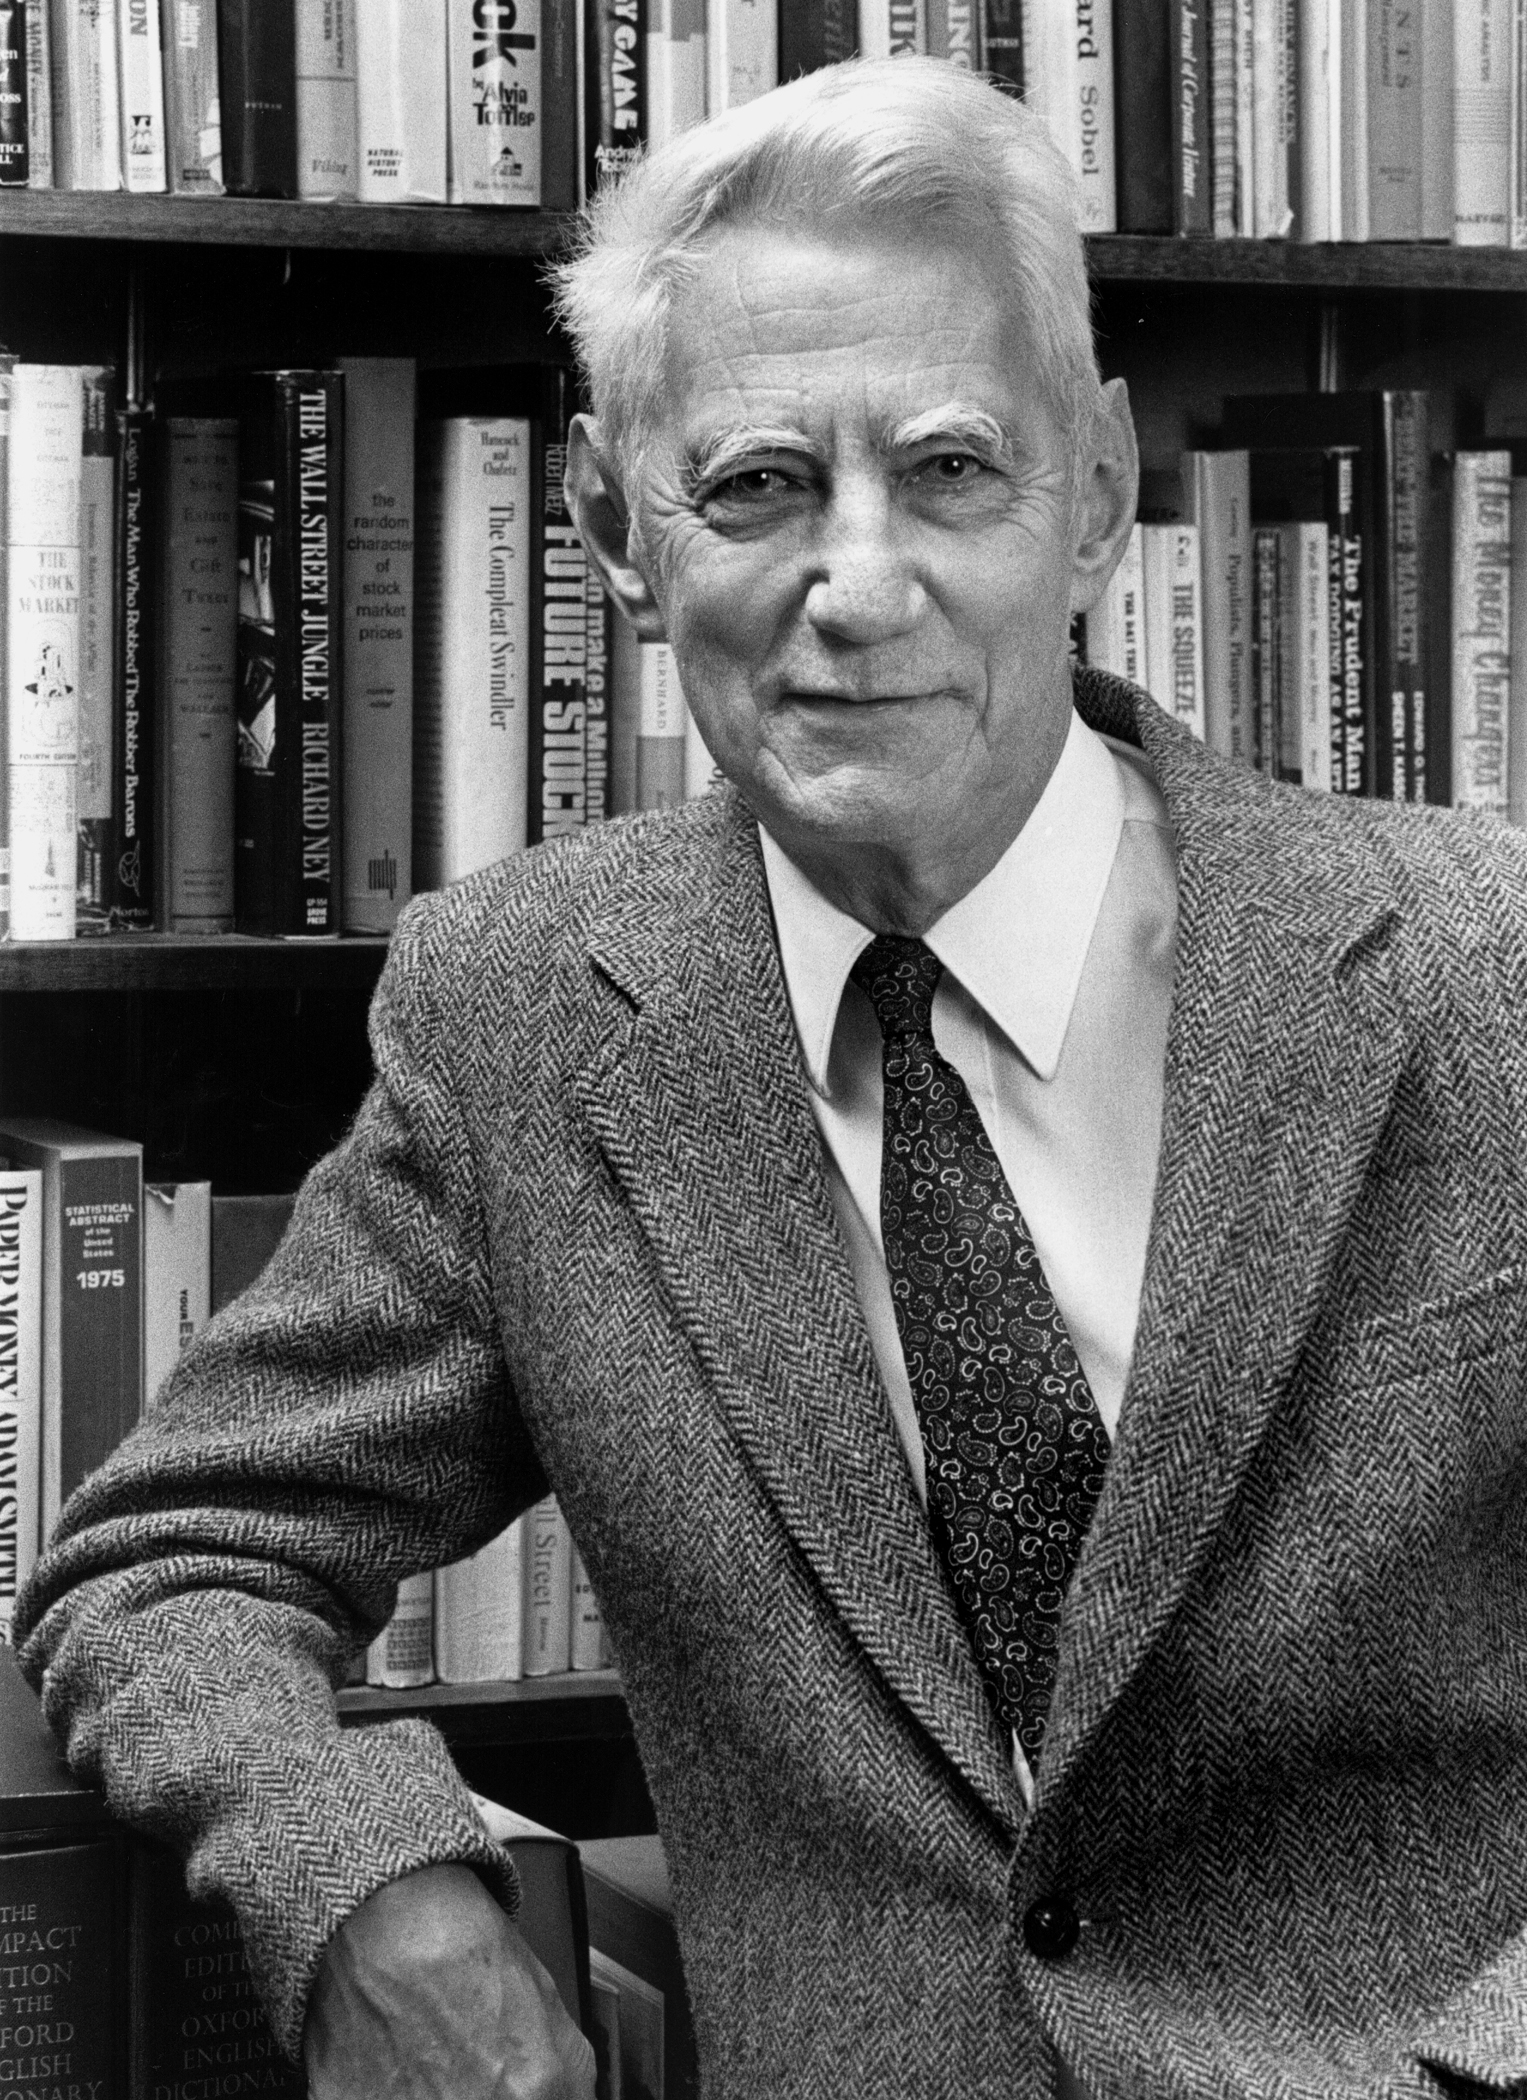
\includegraphics[width=\linewidth]{imagens/shannon.jpeg}
\\%
\scriptsize{Uso permitido pela Nokia Corporation e AT\&T Archives
(\url{http://www bell-labs com/news/2001/february/26/shannon2_lg.jpeg})}
\end{minipage}
\end{tcolorbox}

Apresentaremos agora sete verdades sobre os bits. Nós chamamos essas verdades de
``koans'': no Zen Budismo um koan é uma anedota ou um enigma verbal paradoxal
utilizado para demonstrar a inadequação de um raciocínio lógico, para provocar
meditação e iluminação. Esses koans são simplificações e generalizações
excessivas. Eles descrevem um mundo que está em desenvolvimento mas que ainda
não emergiu completamente. Mas mesmo hoje eles são mais verdadeiros do que
frequentemente percebemos. Esses temas ecoarão em nossos relatos sobre a
explosão digital.


%%%%%%%%%%%%%%%%%%%%
\subsubsection*{Koan 1: São apenas bits}
Seu computador e seu smartphone (na verdade, apenas outro computador) criam com 
sucesso a ilusão de que contêm fotografias, cartas, músicas e filmes. Na 
realidade, tudo o que eles contêm são bits --- muitos deles --- organizados de
maneiras que você não pode ver. Seu computador foi projetado para armazenar 
apenas bits; todos os arquivos, pastas e diferentes tipos de dados são ilusões 
criadas por programadores de computador. Quando você envia uma mensagem contendo 
uma fotografia, os computadores que lidam com sua mensagem enquanto ela flui 
pela Internet não têm ideia de que estão lidando com parte de texto e parte de 
gráfico. As chamadas telefônicas também são apenas bits, e isso ajudou a criar 
concorrência: empresas telefônicas tradicionais, empresas de telefonia celular, 
empresas de TV a cabo e provedores de serviços de voz sobre IP (VoIP) podem 
trocar bits entre si para concluir chamadas. A Internet foi projetada para lidar 
apenas com bits, não com e-mails ou anexos, que são invenções de engenheiros de 
software. Não poderíamos viver sem esses conceitos mais intuitivos, mas eles são 
artifícios. Por baixo de tudo, são apenas bits.

Este koan é mais importante do que você pode pensar. Considere a história de 
Naral Pro-Choice America e Verizon Wireless. A Naral queria formar um grupo de 
mensagens de texto para enviar alertas aos seus membros. A Verizon decidiu não 
permitir, citando as coisas ``controversas ou desagradáveis'' que as mensagens 
poderiam conter\footnote{Adam Liptak, ``Verizon Blocks Messages of Abortion
Rights Group,'' \textit{The New York Times}, September 27, 2007, \url{https://www.nytimes.com/2007/09/27/us/27verizon.html}.}. Grupos de alerta por mensagem de texto para candidatos 
políticos seriam permitidos, mas não para causas políticas consideradas 
controversas. Se a Naral simplesmente quisesse um serviço telefônico ou um 
número 800, a Verizon não teria escolha. As empresas telefônicas foram 
consideradas ``transportadoras comuns'' há muito tempo. Assim como as ferrovias, 
as empresas telefônicas são legalmente proibidas de selecionar clientes entre 
aqueles que desejam seus serviços. No mundo dos bits, não há diferença entre uma 
mensagem de texto e uma chamada telefônica sem fio. São apenas bits, viajando 
pelo ar por ondas de rádio. Mas a lei não acompanhou a tecnologia. Ela não 
trata todos os bits da mesma forma, e as regras de transporte comum para bits de 
voz não se aplicam aos bits de mensagens de texto.

A Verizon recuou no caso da Naral, mas não em relação ao princípio. Uma empresa 
de telefonia pode fazer o que achar que maximizará seus lucros ao decidir quais 
mensagens distribuir. No entanto, nenhuma distinção de engenharia sensata pode 
ser feita entre mensagens de texto, chamadas telefônicas e quaisquer outros bits 
que viajam pelas ondas digitais.

\begin{tcolorbox}[title={Exclusivos e rivais}]
Economistas diriam que os bits, a menos que sejam controlados de alguma forma, 
tendem a ser não-exclusivos (uma vez que algumas pessoas os possuem, é difícil 
impedi-las de compartilhar com outros) e não-rivalizantes (quando alguém os 
recebe de mim, eu não fico com menos). Em uma carta em que escreveu sobre a 
natureza das ideias, Thomas Jefferson afirmou de forma eloquente essas duas 
propriedades: ``Se a natureza tornou alguma coisa menos suscetível do que todas 
as outras a ser propriedade exclusiva, é a ação do poder de pensamento chamado 
ideia, que um indivíduo pode possuir exclusivamente enquanto a mantiver para si 
mesmo; mas no momento em que é divulgada, ela se impõe a posse de todos, e o 
receptor não pode se despojar dela. Sua característica peculiar, também, é que 
ninguém possui menos, porque todos os outros possuem a totalidade
dela.''\footnote{``Article 1, Section 8, Clause 8: Thomas Jefferson to Isaac
McPherson,'' in Andrew A. Lipscomb and Albert Ellery Bergh, eds., \textit{The
Writings of Thomas Jefferson} (Thomas Jefferson Memorial Association, 1905),
\url{http://press-pubs.uchicago.edu/founders/documents/a1_8_8s12.html}.}
\end{tcolorbox}


%%%%%%%%%%%%%%%%%%%%
\subsubsection*{Koan 2: Perfeição é normal}
Errar é humano. Quando os livros eram laboriosamente transcritos à mão em 
scriptoria antigos e mosteiros medievais, erros se infiltravam a cada cópia. 
Computadores e redes funcionam de maneira diferente. Cada cópia é perfeita. Se 
você enviar uma fotografia por e-mail para um amigo, ele não receberá uma versão 
mais borrada do que a original. A cópia será idêntica, até mesmo em níveis de 
detalhes muito pequenos para serem percebidos pelo olho humano.

É claro que os computadores podem falhar. As redes também podem sofrer 
interrupções. Se a energia acabar sem backup de bateria, nada funciona. 
Portanto, a afirmação de que as cópias são normalmente perfeitas é apenas 
relativamente verdadeira. As cópias digitais são perfeitas apenas na medida em 
que podem ser comunicadas. E sim, teoricamente é possível que um único bit de 
uma mensagem grande chegue incorretamente, mas também é possível que um vulcão 
entre em erupção sob você e você não receba a mensagem. A probabilidade de um 
bit errôneo é menor do que a probabilidade de uma catástrofe física, e isso é 
suficiente para todos os propósitos práticos.

As redes não apenas transferem bits de um lugar para outro. Elas verificam se os 
bits parecem ter sido danificados durante a transmissão e os corrigem ou 
retransmitem se parecerem incorretos. Como resultado desses mecanismos de 
detecção e correção de erros, as chances de um erro real --- por exemplo, um 
caractere errado em um e-mail --- são tão baixas que seria mais sensato nos 
preocuparmos com um meteoro atingindo nosso computador, mesmo que sejam 
improváveis os impactos precisos de meteoros.

O fenômeno das cópias perfeitas mudou drasticamente a lei, como é contado no
Capítulo 6, ``Equilíbrio Derrubado''. Nos tempos em que a música era distribuída
em fita cassete, os adolescentes não eram processados por fazer cópias de 
músicas, porque as cópias não eram tão boas quanto as originais, e as cópias das 
cópias seriam ainda piores. A razão pela qual as pessoas hoje em dia preferem 
mais assinar serviços de música do que possuir suas próprias cópias das 
gravações é que as cópias são perfeitas --- não apenas tão boas quanto a 
original, mas idênticas à original, de forma que até mesmo a noção de
``original'' é insignificante. As consequências da interrupção digital da
``propriedade intelectual'' ainda não acabaram. Os bits são uma espécie peculiar 
de propriedade. Uma vez que eu os libere, todos os têm. E se eu lhe der meus 
bits, eu não tenho menos deles.


%%%%%%%%%%%%%%%%%%%%
\subsubsection*{Koan 3: Há carência no meio da abundância}
Por mais que o armazenamento de dados em todo o mundo seja grande hoje, daqui a
dois anos ele será o dobro. No entanto, a explosão de informações significa, 
paradoxalmente, a perda de informações que não estão online. Um de nós viu um 
médico novo em uma clínica que ele usava há décadas. Ela mostrou a ele gráficos 
detalhados da química do seu sangue, dados transferidos do dispositivo médico 
doméstico para o computador da clínica --- mais dados do que qualquer 
especialista poderia ter tido à disposição há cinco anos. O médico então 
perguntou se ele já havia feito um teste de estresse e o que o teste havia 
mostrado. Esses registros deveriam estar lá, explicou o paciente, no prontuário 
médico. Mas as informações estavam no arquivo em \textbf{papel}, ao qual o 
médico não tinha acesso. Não estava na memória do \textbf{computador}, e a
memória do paciente estava sendo usada como um substituto inadequado. Os dados
antigos poderiam muito bem não ter existido, já que não eram digitais.

Mesmo as informações que existem em formato digital são inúteis se não houver 
dispositivos para lê-las. O rápido progresso da engenharia de armazenamento fez 
com que os dados armazenados em dispositivos obsoletos deixassem de existir 
efetivamente. Uma versão digital criada no século XX para o ``The Domesday Book''
britânico do século XI, mostrado na Figura~\ref{fig:domesday}, já era inútil
quando tinha apenas um sexagésimo da idade do original\footnote{Robin McKie and
Vanessa Thorpe, ``Digital Domesday Book lasts 15 years not 1000,''
\textit{Guardian Unlimited}, March 3, 2002.}.

\begin{figure}[h]
\centering
\caption{The Domesday Book de 1806.}
\label{fig:domesday}
\vspace{-0.3cm}
%\fbox{
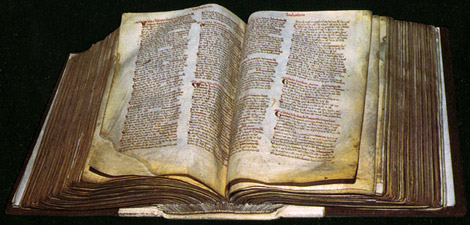
\includegraphics[scale=0.5]{imagens/domesday.jpg}
%}
\\
\scriptsize{UK National Archives
(\url{https://www.worldhistory.org/image/9476/great-domesday-book/}). Uma versão
digital comemorativa do 900º aniversário não podia ser mais lida 15 anos após
o lançamento.}
\end{figure}

Ou considere a busca, um dos assuntos do Capítulo 4, ``Guardiões''. No início,
os motores de busca, como o Google, eram conveniências interessantes que algumas
pessoas usavam para fins especiais. Com o crescimento da World Wide Web e a 
explosão de informações online, os motores de busca se tornaram o primeiro lugar 
onde muitas pessoas procuram por informações --- antes mesmo de consultarem
livros ou perguntarem a amigos. Aparecer em destaque nos resultados de busca se
tornou uma questão de vida ou morte para as empresas. Podemos passar a comprar 
de um concorrente se não encontrarmos o site que queríamos logo nas primeiras 
páginas de resultados. Podemos presumir que algo não aconteceu se não 
conseguirmos encontrá-lo --- rapidamente --- em uma fonte de notícias online.
Se algo não pode ser encontrado rapidamente, é como se não existisse de forma
alguma.

E algumas informações não são verdadeiras. Todos os mecanismos que permitem a
comunicação e o armazenamento de fatos também funcionam para falsidades. A 
feiúra e a crueldade são capturadas tão facilmente em bits quanto a beleza e a 
bondade. A economia de mercado da informação muda quando todos podem ser 
editores e ninguém precisa de um editor. Inundações de desinformação, informação 
falsa e lixo podem sobrecarregar a verdade e a beleza. Sociedades autoritárias 
podem ser capazes de gerenciar o fluxo de bits de forma mais eficiente do que 
sociedades livres, que correm o risco de serem minadas por seus próprios 
princípios de liberdade de informação.


%%%%%%%%%%%%%%%%%%%%
\subsubsection*{Koan 4: Processamento é poder}

A velocidade de um computador geralmente é medida pelo número de operações 
básicas, como adições, que podem ser realizadas em um segundo. Os computadores 
mais rápidos disponíveis no início dos anos 1940 conseguiam realizar cerca de 
cinco operações por segundo. Os mais rápidos de hoje podem realizar cerca de um 
trilhão. Compradores de computadores pessoais sabem que uma máquina que parece 
rápida hoje parecerá lenta daqui a um ano ou dois.

Por pelo menos três décadas, o aumento na velocidade dos processadores era 
exponencial. Os computadores ficavam duas vezes mais rápidos a cada dois anos. 
Esses aumentos eram uma consequência da Lei de Moore.

\begin{tcolorbox}[title={Lei de Moore}]
Gordon Moore, fundador da Intel Corporation, observou que a densidade dos 
circuitos integrados parecia dobrar a cada dois anos. Essa observação é 
conhecida como ``Lei de Moore''. Claro, não é uma lei natural, como a lei da
gravidade. Em vez disso, é uma observação empírica do progresso da engenharia e 
um desafio aos engenheiros para continuarem sua inovação. Em 1965, Moore previu 
que esse crescimento exponencial continuaria por muito tempo\footnote{G. E.
Moore, ``Cramming More Components onto Integrated Circuits,'' \textit{Proceedings
of the IEEE 86}, no. 1 (January 1998): 82--85, \url{https://doi.org/10.1109/JPROC.1998.658762}.}.
O fato de ter continuado por mais de 40 anos é uma das grandes maravilhas da
engenharia. Nenhum outro esforço na história sustentou uma taxa de crescimento
nem perto dessa.
\end{tcolorbox}

Desde 2001, a velocidade do processador não tem seguido a Lei de Moore; na 
verdade, os processadores mal ficaram mais rápidos. Mas isso não significa que 
os computadores não continuarão a ficar mais rápidos. Novos projetos de chips 
incluem vários processadores no mesmo chip, para que o trabalho possa ser 
dividido e executado em paralelo. Essas inovações de design prometem alcançar o 
mesmo efeito que aumentos contínuos na velocidade bruta do processador. E as 
mesmas melhorias tecnológicas que tornam os computadores mais rápidos também os 
tornam mais baratos.

O rápido aumento na capacidade de processamento significa que as invenções saem 
dos laboratórios e entram rapidamente nos bens de consumo. Aspiradores de pó 
robóticos e veículos com estacionamento automático eram teoricamente possíveis 
há uma década, mas agora se tornaram produtos de consumo. Tarefas que hoje 
parecem exigir habilidades exclusivamente humanas não são mais apenas objeto de 
projetos de pesquisa em laboratórios corporativos ou acadêmicos; elas estão 
incorporadas em produtos de consumo. Reconhecimento facial e reconhecimento de 
voz estão aqui e agora; telefones sabem quem está ligando, e câmeras de 
vigilância não precisam de humanos para observá-las. O poder vem não apenas dos 
bits, mas da capacidade de fazer coisas com os bits.


%%%%%%%%%%%%%%%%%%%%
\subsubsection*{Koan 5: Mais do mesmo pode ser uma coisa totalmente nova}
O crescimento explosivo é um crescimento exponencial --- dobrando em uma taxa 
constante. Imagine ganhar 100\% de juros anuais em sua conta poupança: em 10 
anos, seu dinheiro teria aumentado mais de mil vezes, e em 20 anos, mais de um 
milhão de vezes. Uma taxa de juros mais razoável de 5\% atingirá os mesmos 
pontos de crescimento, mas o fará 14 vezes mais lentamente. Epidemias 
inicialmente se espalham de forma exponencial, à medida que cada pessoa 
infectada infecta várias outras.

Quando algo cresce exponencialmente, por um longo tempo pode parecer que não 
está mudando. Se não o observarmos constantemente, parecerá que ocorreu algo 
descontínuo e radical enquanto não estávamos olhando.

É por isso que as epidemias no início passam despercebidas, independentemente de
quão catastróficas possam ser quando estão em pleno andamento. Imagine uma
pessoa doente infectando duas pessoas saudáveis, e no dia seguinte cada uma
dessas duas infecta mais duas, e no dia seguinte cada uma dessas quatro infecta 
mais duas, e assim por diante. O número de novas infecções cresce de 2 para 4 
para 8. Em uma semana, 128 pessoas contraem a doença em um único dia, e o dobro 
desse número agora está doente, mas em uma população de 10 milhões, ninguém 
percebe. Mesmo depois de duas semanas, apenas cerca de 3 pessoas em 1.000 estão 
doentes. Mas após mais uma semana, 40\% da população está doente e a sociedade 
entra em colapso. A pandemia de coronavírus de 2019--2020 seguiu mais ou menos 
esse padrão em partes do mundo onde as sociedades não reagiram rapidamente. No 
início da epidemia em Wuhan, o número de casos dobrava aproximadamente a cada 
três dias\footnote{Steven Sanche et al., ``High Contagiousness and Rapid Spread
of Severe Acute Respiratory Syndrome Coronavirus 2,'' \textit{Emerging
Infectious Diseases} 26, no. 7 (July 2020): 1470--1477,
\url{https://dx.doi.org/10.3201/eid2607.200282.}}.

O crescimento exponencial é na verdade suave e constante; leva muito pouco 
tempo para passar de uma mudança imperceptível para algo altamente visível. O 
crescimento exponencial de qualquer coisa pode fazer o mundo parecer 
completamente diferente do que era antes. Quando esse limiar é ultrapassado, 
mudanças que são ``apenas'' quantitativas podem parecer qualitativas.

Outra maneira de entender a aparente abruptidão do crescimento exponencial ---
sua força explosiva --- é pensar em quão pouco tempo temos para responder a ele.
Nossa epidemia hipotética levou três semanas para sobrecarregar a população. Em 
que ponto ela era apenas metade tão devastadora? A resposta \textbf{não} é ``uma
semana e meia''. A resposta é no \textbf{penúltimo} dia. Suponha que levasse uma
semana para desenvolver e administrar uma vacina. Então, perceber a epidemia
após uma semana e meia deixaria tempo de sobra para evitar o desastre. Mas isso
exigiria compreender que \textbf{havia} uma epidemia quando apenas 2.000 pessoas
em 10 milhões estavam infectadas.

A história da informação está repleta de exemplos de mudanças não percebidas 
seguidas por explosões deslocadoras. Aqueles com a visão de futuro para notar a 
explosão apenas um pouco mais cedo do que todos os outros podem obter benefícios 
enormes. Aqueles que se movem um pouco mais devagar podem ser sobrecarregados 
quando tentam responder. Tome o caso da fotografia digital.

Em 1983, os compradores de Natal podiam comprar câmeras digitais para conectar 
aos seus computadores domésticos IBM PC e Apple II. O potencial estava lá para 
qualquer um ver; não estava escondido em laboratórios corporativos secretos. Mas 
a fotografia digital não decolou. Economicamente e praticamente, não era viável.
As câmeras eram muito volumosas para caber no bolso, e as memórias digitais eram
muito pequenas para armazenar muitas imagens. Mesmo 14 anos depois, a fotografia
em filme ainda era uma indústria robusta. No início de 1997, as ações da Kodak
atingiram um preço recorde, com um aumento de 22\% no lucro trimestral, 
``impulsionado pelas vendas saudáveis de filmes e papel\ldots\ [e] pelo negócio
de filmes de cinema'', de acordo com um relatório de notícias\footnote{``Kodak,
GE, Digital Report Strong Quarterly Results,'' \textit{Atlanta Constitution},
January 17, 1997.}. A empresa aumentou seu dividendo pela primeira vez em oito
anos. Mas em 2007, as memórias digitais haviam se tornado enormes, os 
processadores digitais haviam se tornado rápidos e compactos, e ambos eram 
baratos. Como resultado, as câmeras se tornaram pequenos computadores. A empresa 
que um dia foi sinônimo de fotografia era apenas uma sombra do que já foi. A 
Kodak anunciou que seu quadro de funcionários seria reduzido para 30.000, pouco 
mais de um quinto do tamanho que tinha nos bons tempos do final dos anos
1980\footnote{Claudia H. Deutsch, ``Shrinking Pains at Kodak,'' \textit{The New
York Times}, February 9, 2007.}. Em 2018, esse número estava em cerca de 5.400.
Bits tiraram 90\% dos empregos. A Lei de Moore avançou mais rapidamente do que a
Kodak.

No mundo em rápida mudança dos bits, vale a pena notar até mesmo pequenas
mudanças e fazer algo a respeito delas.


%%%%%%%%%%%%%%%%%%%%
\subsubsection*{Koan 6: Nada vai embora}

